\documentclass[a4paper,12pt]{article}
\usepackage[utf8]{inputenc}
\usepackage[T2A]{fontenc}
\usepackage[english,russian]{babel}
\usepackage{natbib}
\usepackage{graphicx}
\usepackage{amsmath}
\usepackage{pgfplots}
\usepackage{color} %% это для отображения цвета в коде
\usepackage{listings} %% собственно, это и есть пакет listings
\usepackage{caption}
\usepackage{indentfirst} % Красная строка
\DeclareCaptionFont{white}{\color{white}} %% это сделает текст заголовка белым
%% код ниже нарисует серую рамочку вокруг заголовка кода.
\DeclareCaptionFormat{listing}{\colorbox{white}{\parbox{\textwidth}{#1#2#3}}}
\captionsetup[lstlisting]{format=listing,labelfont=black,textfont=black}

\title{Министерство образования Российской Федерации
Московский Государственный Технический Университет им. Н.Э. Баумана}
\author{Мхитарян Виктория}
\date{Москва, 2018}

%%%%%%%%%%%%%%%%%%%%%%%%%%%%%%%%%%%%%%%%%%%%%%%%%%%%%%%%%%%%%%%%%%%%%%%%%%%%%%%%%%%%%%%%%%%%%%%

\begin{document}
\lstset{ %
language=C,                 % выбор языка для подсветки
basicstyle=\small\sffamily, % размер и начертание шрифта для подсветки кода
numbers=left,               % где поставить нумерацию строк (слева\справа)
numberstyle=\tiny,           % размер шрифта для номеров строк
stepnumber=1,                   % размер шага между двумя номерами строк
numbersep=5pt,                % как далеко отстоят номера строк от подсвечиваемого кода
backgroundcolor=\color{white}, % цвет фона подсветки - используем \usepackage{color}
showspaces=false,            % показывать или нет пробелы специальными отступами
showstringspaces=false,      % показывать или нет пробелы в строках
showtabs=false,             % показывать или нет табуляцию в строках
frame=false,              % рисовать рамку вокруг кода
tabsize=1,                 % размер табуляции по умолчанию равен 2 пробелам
captionpos=t,              % позиция заголовка вверху [t] или внизу [b] 
breaklines=true,           % автоматически переносить строки (да\нет)
breakatwhitespace=false, % переносить строки только если есть пробел
escapeinside={\%*}{*)}   % если нужно добавить комментарии в коде
}
\thispagestyle{empty}

\begin{figure}[th]
\noindent\centering{
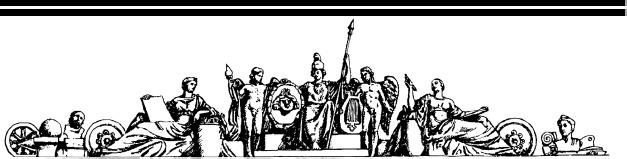
\includegraphics[scale = 0.6]{img-AFYrS7.jpg}}
\end{figure}

\begin{center}
    {\Large Министерство образования Российской Федерации\\
Московский Государственный Технический\\ Университет им. Н.Э. Баумана \\[66pt]
Отчет по лабораторной работе №6 \\
По курсу «Анализ алгоритмов»}
\end{center}

\begin{center}
    {\LARGE \textbf{Тема: «Конвейер»\\[90pt]}}
\end{center}

\begin{flushright}
Студент: {\bfVМхитарян В.К.}\\ Группа: {\bfИУ7-54}\\[20pt] 
Преподаватель: {\bfПогорелов Д.А.}\\[80pt]
\end{flushright}

\begin{center}
    {\Large Москва, 2018}
\end{center}

\newpage

\tableofcontents

%%%%%%%%%%%%%%%%%%%%%%%%%%%%%%%%%%%%%%%%%%%%%%%%%%%%%%%%%%%%%%%%%%%%%%%%%%%%%%%%%%%%
\newpage
\section*{Введение}
\addcontentsline{toc}{section}{Введение}

Целью данной лабораторной работы является применение конвейерной обработки данных. Конвейерная обработка данных может быть полежной, когда каждая операция занимает много времени. В данной работе будет рассмотрена задача заполнения массива случайными числами, вычисление суммы элементов массива и запись результата в файл.
%%%%%%%%%%%%%%%%%%%%%%%%%%%%%%%%%%%%%%%%%%%%%%%%%%%%%%%%%%%%%%%%%%%%%%%%%%%%%%%%%%%
\newpage
\section*{1. Аналитическая часть}
\addcontentsline{toc}{section}{1. Аналитическая часть}

В данном разделе будут приведены теоретические сведения о алгоритмах, их описание и разбор.

\subsection*{1.1. Описание алгоритмов}
\addcontentsline{toc}{subsection}{1.1. Описание алгоритмов}

Для реализации конвейерной обработки с помощью потоков было выделено три этапа, на каждом из которых производится своя операция обработки данных. В первом потоке выполняется первая операция (заполнение массива случайными числами), после чего выходные данные передаются во второй поток для выполнения второй операции (вычисление суммы элементов массива). Выходные данные после выполнения третьей операции подаются в третий поток для выполнения третьей операции (запись результата в файл).\\


\newpage
\section*{2. Конструкторская часть}
\addcontentsline{toc}{section}{2. Конструкторская часть}
В данном разделе будет рассмотрен способ организации конвейера.

\subsection*{2.1. Способ организации конвейера}
\addcontentsline{toc}{subsection}{2.1. Способ организации конвейера}
Конвейер состоит из 3х потоков для 3х последовательных задач и 4х очередей. Сначала, id массивов, которые необходимо обработать, заносятся в очередь ${Q_0}$. Из очереди ${Q_0}$, если она не пуста и первый поток свободен, достается элемент, который и передается в первый поток. 

В первом потоке с указанным id создается матрица, заполненная случайным образом, и находится ее обратная матрица. После выполнения действий над текущим элементом первый поток добавляет, осуществляя монополизированный доступ к переменной очереди ${Q_1}$, помещает результат выполнения операции в очередь ${Q_1}$. 

Далее, по аналогии с первым потоком, второй поток извлекает из очереди ${Q_1}$ элемент, производит над ним вычисления (возведение матрицы в квадрат) и заносит результат в очередь ${Q_2}$. Аналогично с третьим потоком.
Процесс заканчивается, когда в очереди ${Q_3}$ (очереди полностью готовых элементов) аккумулируется столько же элементов, сколько поступило на вход. \\


\newpage
\section*{3. Технологическая часть}
\addcontentsline{toc}{section}{3. Технологическая часть}

В данном разделе будет описаны требования к программному обеспечению, средства реализации и листинг кода.

\subsection*{3.1. Требования к программному обеспечению}
\addcontentsline{toc}{subsection}{3.1. Требования к программному обеспечению}
Минимальные системные требования: PC с операционной системой  Windows 7, MacOS X или Linux(Ubuntu). Процессор с частотой 2.0GHz или выше. С оперативной памятью не менее 2 Гб. Требуются устройства ввода: клавиатура, мышь.

\subsection*{3.2. Средства реализации}
\addcontentsline{toc}{subsection}{3.2. Средства реализации}
В данной работе был выбран открытый мультипарадигмальный компилируемый язык программирования С++. С++ является одним из самых популярных языков программирования и имеет огромную область применения. Среда для разработки выбрана CLion.

\subsection*{3.3. Листинг кода}
\addcontentsline{toc}{subsection}{3.2. Листинг кода}




\begin{lstlisting}[label=some-code,caption=Конвейер]
while (q[2].size() != OBJ_COUNT) {
        if (current_element < OBJ_COUNT) {
            Array array(ARRAY_SIZE, obj[current_element]);
            queue1.push(array);
            current_element++;
        }

        // Level 1
        if (threads[0].joinable())
            threads[0].join();
        if (!queue1.empty() && !threads[0].joinable()) {
            Array front_array = queue1.front();
            queue1.pop();

            auto level1 = [](Array obj, queue<Array> &queue) {
                obj.rand_vec();

                mutex queue_mutex;
                queue_mutex.lock();
                queue.push(obj);
                queue_mutex.unlock();
            };

            threads[0] = thread(level1, front_array, ref(q[0]));
        }

        // Level 2
        if (threads[1].joinable()){
            threads[1].join();
        }
        if (!q[0].empty() && !threads[1].joinable()) {
            Array front_array = q[0].front();
            q[0].pop();

            auto level2 = [](Array obj, queue <Array> &queue) {
                obj.summa();

                mutex queue_mutex;
                queue_mutex.lock();
                queue.push(obj);
                queue_mutex.unlock();
            };

            threads[1] = thread(level2, front_array, ref(q[1]));
        }

        // Level 3
        if (threads[2].joinable()){
            threads[2].join();
        }
        if (!q[1].empty() && !threads[2].joinable()) {
            Array front_array = q[1].front();
            q[1].pop();

            auto level3 = [](Array obj, queue <Array> &queue) {
                string str = "file" + to_string(obj.get_id()) + ".txt";
                obj.print(str);

                mutex queue_mutex;
                queue_mutex.lock();
                queue.push(obj);
                queue_mutex.unlock();
            };

            threads[2] = thread(level3, front_array, ref(q[2]));
        }
    }
\end{lstlisting}



\begin{lstlisting}[label=some-code,caption=Класс Array]
class Array {
private:
    std::vector<int> array;
    int length;
    int id;

    void timeout() {
        int wait_time = rand()%2000;
        std::this_thread::sleep_for(std::chrono::nanoseconds(wait_time));
    }

public:
    Array(int length, int id) {
        this->length = length;
        this->id = id;
        for (int i = 0; i < length; ++i) {
            array.push_back(0);
        }
    };

    void rand_vec() {
        timeout();

        for (int i = 0; i < length; ++i) {
            array[i] = rand()%1000;
        }
    }

    void summa() {
        timeout();
        int sum = 0;
        for (int i = 0; i < length; i++){
            sum += array[i];
        }
        array[0] = sum;
    }

    void print(std::string file_name) {
        std::ofstream file (file_name);

        timeout();

        file << "Summa: ";
        file << array[0];
        file << "\n";
    }
    
    int get_id() {
        return id;
    }
};
\end{lstlisting}


\newpage
\section*{4. Эксперементальная часть}
\addcontentsline{toc}{section}{4. Эксперементальная часть}

В данном разделе будут приведены эксперименты и сравнительный анализ алгоритмов на основе приведенных данных.

\subsection*{4.1. Постановка эксперимента}
\addcontentsline{toc}{subsection}{4.1. Постановка эксперимента}

Задачей этого эксперимента является сравнение эффективности последовательного выполнения команд и конвейерной обработки. Будет проведет анализ на основе тестов.

\subsection*{4.2. Сравнительный анализ на материале экспериментальных данных}
\addcontentsline{toc}{subsection}{4.2. Сравнительный анализ на материале экспериментальных данных}

Измерения проводились для целочисленных массивов постоянной величины равной 500 с помощью библиотеки std::chrono. Значения в таблицах представлены в наносекундах(среднее из 10 замеров).



\begin{flushright}Таблица 1. Результаты замеров времени.\end{flushright}
\begin{center}
\begin{tabular}{|c|c|c|}
\hline
 & Конвейер & Последовательно\\
\hline
\hline
100&54686477&111191164\\
\hline
200&120387625&130504283\\
\hline
300&394637157&530076330\\
\hline
400&393970683&1026480147\\
\hline
500&674612983&1474704303\\
\hline
600&753455103&1335335403\\
\hline
700&887185877&1868453597\\
\hline
800&1151811773&1661585940\\
\hline
900&1475499240&2319997067\\
\hline
1000&1203419145&2160687625\\
\hline
\end{tabular}
\end{center}

\newpage
Представление тестовых данных из таблицы 1.

\begin{figure}[ht]
\noindent\centering{
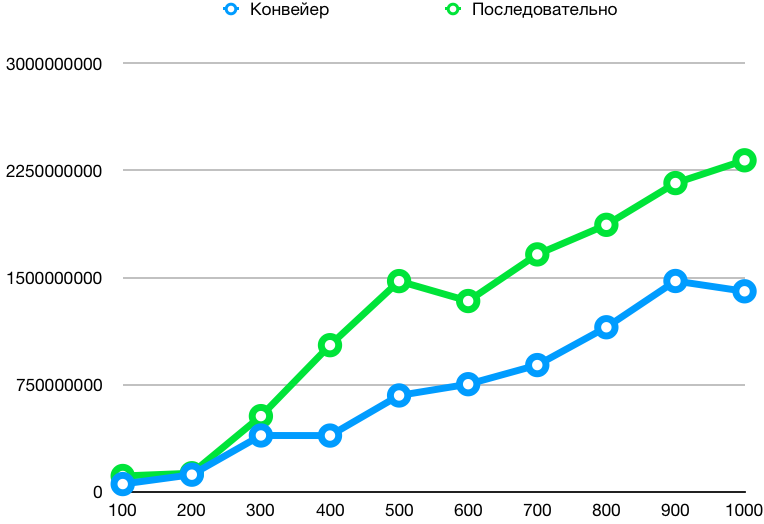
\includegraphics[scale = 0.6]{Chart.png}
\end{figure}

По результатам проведенного эксперимента можно сделать вывод, что выполнение конвейерной обработкой эффективнее чем последовательной. В данном примере конвейерная реализация при разделении на 3 этапа дает прирост в производительности примерно в 2 раза.


\newpage
\addcontentsline{toc}{section}{Заключение}
{\Large\bfЗаключение\\}

В ходе проведенной работы, были изучена и реализована конвейерная обработка данных на языке программирования С++. Были получены навыки работы с потоками и mutex. Было выполнено сравнение последовательных вычислении и конвейерной обработки.

\end{document}